\documentclass[11pt]{article}
\usepackage{graphicx,natbib,amsmath,color,matlab-prettifier,listings,epstopdf}
\title{SEIR Modelling COVID-19 to Analyse Government Strategies in the UK}
\author{Deniz Dilan Dogan}
\begin{document}
	\maketitle
	\tableofcontents
\pagebreak
\section{Introduction and Overview}
\subsection{Introduction to pandemic}
During late December in 2019 Wuhan Municipal Health Commission, reported to the World Health Organization a series of pneumonia cases, all in which the causal agent was unknown. The number of patients which had adjacent symptoms became significant enough for WHO to investigate this report further using information collected from authorities in Wuhan. Soon after, China publicised the genetic sequence of COVID-19, known as the novel coronavirus at the time. This was immediately followed by the inevitable first recorded case outside of China occurred during mid-January in Thailand. The patient had been travelling from Wuhan combining this new case with information gathered from the first bunch of patients, it strongly implied human-to-human transmission, in turn WHO acknowledged that there was a potential for an outbreak. After months of analysing data, strategizing with experts globally, devising plans and support systems to contain the virus, the cases had only increased exponentially. On the 11th of March, with over 118,000 cases globally and 4,291 resulting fatalities, WHO announced that COVID-19 fulfilled the required criteria to be classed as a pandemic\citep{WHO'stimelineofCOVID-19}.  \par
Since this date the UK government has implemented various strategies to contain the virus. But how effective were/are these strategies if effective at all? The aim of this piece is to analyse and compare strategies used by the UK Government during the current global pandemic, using the SEIR model to determine how lockdowns and general rules have affected fatalities and general transmission of COVID-19. Hence, we can explore the significance of these strategies and in turn the validity of statements made by officials and by the general public.
\subsection{Why modelling of a pandemic is necessary}
Modelling infectious diseases is highly important as it is the gateway to forecasting how diseases will spread with respect to time. Just like weather forecasting, this allows people to live accordingly and plan accordingly to what is predicted to happen soon. To respond to a new outbreak, we need to know the severity of the said outbreak i.e., how quickly it is spreading, and how quickly it will spread. If we had no way of measuring the severity of an outbreak, we would have trouble identifying a pandemic to begin with and the most appropriate course of action to contain the said pandemic. Hence, we would have to react to all out breaks in the same way for the sake of consistency, which is unsustainable socially and economically. \par
An early example of compartmental modelling being used to control a pandemic is given by the work of Sir Ronald Ross in 1902 on the transmission of malaria between mosquitos and humans. He concluded that reducing the population of mosquitos below a critical level can contain the spread of malaria, since it’s extremely hard to control the population of mosquitos this could not be applied for all populations but in the cases where it was applicable, it worked as the model predicted which in turn lead to his Nobel Prize in Medicine\citep{brauer2019introduction}. Although, it is important to note mathematical models are not perfect, they have a set of limitations that are created due to assumptions made to simplify the model and make it accessible. Even though they are not perfect, as shown by Sir Ronald Ross’ work, they tend to make good predictions that can help us contain outbreaks.
\section{The Model}
\subsection{Why is this variant of SIR modelling}
This model is appropriate for the COVID-19 pandemic as it allows consideration of the latency period, which is the period between contracting the infection and then becoming infectious and the incubation period which is the period between becoming infectious and showing symptoms. The latency period and the incubation period combined is the lag between contact of susceptible and infectious, infection and symptoms. This lag is represented by the exposed category. The potential to spread when symptoms have not been present yet is extremely low, to the point of insignificance i.e., the showing of symptoms naturally greatly increases the risk of spread \citep{ spreadofCOVID-19}, hence there is no transmission considered due to contact of susceptible and exposed which will be outlined in the assumptions of this model. Since this model is with respect to time and the lag between infection and symptoms is sufficiently large\citep{10.1093/cid/ciab746} it is important to reflect this in the model to predict the spread as accurately as possible. \par
In the case where the exposed category was not implemented in these models, we would observe a peak at a much earlier day during the pandemic. Which would not affect the comparisons but will affect the overall accuracy of the model, which as crucial to the conclusions of this project considering the analysis of strategies will factor in the day of peak infections. 
\subsection{Assumptions}
	\begin{enumerate}
	    \item The population stays constant i.e., the death rate and birth rate are approximately equivalent.
	    \item Every individual is in the exposed category for the same length of time which is fixed, i.e. infected people will not be infectious with symptoms until 5.8 days \citep{10.1093/cid/ciab746}.
	    \item All individuals are equally susceptible to COVID-19, and the whole population is considered susceptible at the start of the pandemic.
               \item Individuals that are recovered cannot be reinfected i.e., immunity is assumed.
               \item There is no heterogeneity between individuals i.e., this model ignores network differences between individuals. 
               \item The majority of the population lives in accordance to government guidelines.
               \item Population of the UK is equally distributed, population structure is uniform.
               \item The rate of transmission of COVID-19 is fixed for each 'strategy'.
               \item The removal rate is constant and does not depend on strategy used.
               \item People are infectious with symptoms for 7 days\citep{he2020temporal}.
               \item Hospital patients are 'removed' from hospital in 8.4 days\citep{vekaria2021hospital}.
               \item ICU patients are 'removed' from critical care in 12.4 days\citep{vekaria2021hospital}. 
               \item Exposed people cannot spread COVID-19.
	\end{enumerate}
\subsection{Variables}
$S$: Number of people susceptible to COVID-19 in the UK
 \newline  $E$: Number of Exposed people in the UK
 \newline  $I$: Number of people infectious with COVID-19 with symptoms in the UK
 \newline  $H$: Number of non-ICU hospital patients with COVID-19 in the UK
 \newline  $H_{ICU}$: Number of people admitted to the ICU due to COVID-19 in the UK
 \newline  $R$: Number of people removed by COVID-19 i.e. deceased or recovered in the UK\par
The variables $H$ and $H_{ICU}$ are important when defining a good strategy. I have defined a good strategy as one that controls hospitalisations such that the number of people in hospital does not go over NHS capacity. This capacity is given by the number of hospital beds available in the UK \citep{HBEDS}. There is a different number of beds for ICU patients as they require more sophisticated medical equipment for treatment, hence why hospitalisations are split into to 2 variables. If hospitalisations for COVID-19 go over the capacity or even close to the capacity, this means that people receiving treatment for other diseases will be in danger of delayed treatment whether this be surgery or check-ups that could make the difference between life and death. Acknowledging my model does not consider population structure, the true peak(s) will be much less than predicted by my model. Hence, when analysing the models take them as the worst-case models.
\subsection{Parameters}
$ \alpha_1$: Rate of transmission of COVID-19 to susceptibles by infectious people
\newline $ \alpha_2$: Rate of transmission of COVID-19 to susceptibles by non-ICU patients in the hospital
\newline$ \alpha_3$: Rate of transmission of COVID-19 to susceptibles by people in the ICU
\newline$ \beta$: Rate of transition of exposed to infectous
\newline $ \gamma_1 $: Rate of transition of infectous people to non-ICU patients
\newline $ \gamma_2 $:  Rate of admissions to ICU
\newline $ \delta_1$: Rate of removal of infectious people
\newline $ \delta_2$: Rate of removal of non-ICU patients in hospital
\newline $ \delta_3$: Rate of removal of ICU patients  \par
\subsection{System of differential eqations}
\begin{equation}
\begin{aligned}
\frac{dS}{dt}&=- \alpha_1 SI - \alpha_2 SH - \alpha_3 SH_{ICU} \\
\frac{dE}{dt}&= \alpha_1 SI + \alpha_2 SH + \alpha_3 SH_{ICU} - \beta E \\
\frac{dI}{dt}&= \beta E -\gamma_1 I -\delta_1 I \\
\frac{dH}{dt}&= \gamma_1 I - \gamma_2 H -\delta_2 H \\
\frac{dH_{ICU}}{dt}&= \gamma_2 H -\delta_3 H_{ICU} \\
\frac{dR}{dt}&=\delta_1 I + \delta_2 H + \delta_3 H_{ICU} \\
\end{aligned}
\end{equation} 
\subsection{Flowchart of the system}
\begin{center}
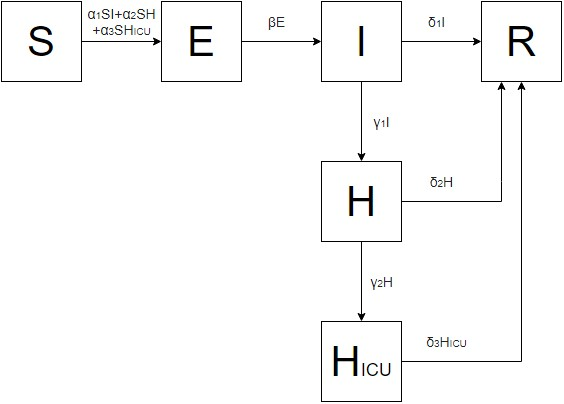
\includegraphics[width=1\textwidth]{SEIHR.jpg} 
\end{center}

\subsection{Calculating parameters using data}
$\alpha_1$, $\alpha_2$, $\alpha_3$ are calculated using the reproductive number given by the data source, the population of the UK and the duration of sickness in days. They are all doubled in value considering that although the whole population is susceptible at the start this decreases very quickly as people are infected, also considering one person does not have potential to spread to the whole population. By assumption $10$ one is infectious with symptoms for 7 days before removal which gives $\alpha_1=\frac{2R_0}{7N}$. By assumption $11$ one is hospitalised for $8.4$ days before removal which gives $\alpha_2=\frac{2R_0}{8.4N}$. By assumption $12$ one is hospitalised in the ICU for $12.4$ days before removal which gives $\alpha_3=\frac{2R_0}{12.4N}$ where N is the population of the UK and $R_0$ varies depending on environment. \par
$\beta$ is calculated using assumption $2$ since these models are with respect to time, the unit of time being days and everyone in the exposed category enters the infectious with symptoms category in 5.8 days, $\beta=\frac{1}{5.8}$ for all environments. \par
In the same way $\delta_1$, $\delta_2$, $\delta_3$ are calculated using the duration of stay in days in given category. By assumption $10$ $\delta_1=\frac{1}{7}$, by assumption $11$ $\delta_2=\frac{1}{8.4}$, and by assumption $12$ $\delta_3=\frac{1}{12.4}$. \par
$\gamma_1$ and $\gamma_2$ are calculated using data. For $\gamma_1$ the daily hospital admissions over the ongoing cases, and for $\gamma_2$ the daily ICU admissions over the current hospital cases since one cannot go from $I$ directly to $H_{ICU}$. To put it simply, it is the proportion of daily admissions into hospital and ICU.

\subsection{Why the R number is problematic}
The basic reproductive number, $R_0$, generally defined as ‘the average number of secondary cases resulting from a standard primary case in a population that is susceptible entirely’ has implied assumptions. To quantify such an important concept, assumptions must be made to simplify calculations and make it as accessible to the population to use as a reference to measure the severity of the spread. The implied assumptions stem from the fact that this value is an average more specifically average transmissibility between individuals and the average infections caused by the individual ironically this disregards the definition of an individual as they are generalised. Hence, disregards the existence of heterogeneity in the population. This heterogeneity is intrinsic to the spread of COVID-19 as factors such as social networks and super spreaders are the main exacerbators of this spread.
There are many methods to calculate $R_0$, most of produce different values for $R_0$ i.e., values that are inconsistent with each other\citep{breban2007theory}, the main one the general public has been exposed to is calculated using existing contact tracing data to estimate spread\citep{R0calculationBBC}, meaning that it is continuously changing and only applies to the recent past, this is also the reproductive number given by the data used to calculate parameters in my models. This relies on data to be up to date and accurate as strategies are planned around the severity of an outbreak. Unfortunately, with this type of calculation of $R_0$ does not allow government to plan for what is to come, it helps deal with the current severity.
$R_0$ is commonly used as a threshold for determining whether an outbreak will progress into a pandemic. Where $R_0>1$ implies that the outbreak will progress into a pandemic and in turn, $R_0<1$ implies outbreak will be contained. \par
However, there are examples of cases where a disease is contained although $R_0>1$, similarly there are cases where disease persists into an outbreak although $R_0<1$\citep{li2011failure}. In turn using the basic reproductive number as a threshold without further evidence that it holds as a threshold is extremely risky. All the caveats surrounding the calculation of $R_0$ i.e., method of calculation and assumptions the model requires to make the calculation of $R_0$ must be carefully considered\citep{li2011failure}. Many diseases are dependent on factors yet to be applied to models we have access to today. The basic reproductive number has many limitations, but it is the best tool to measure the severity of an outbreak and the effectiveness of strategies applied to control an outbreak.
\section{Modelling the no-policy environment}
\subsection{Overall no-policy environment}
\begin{center}
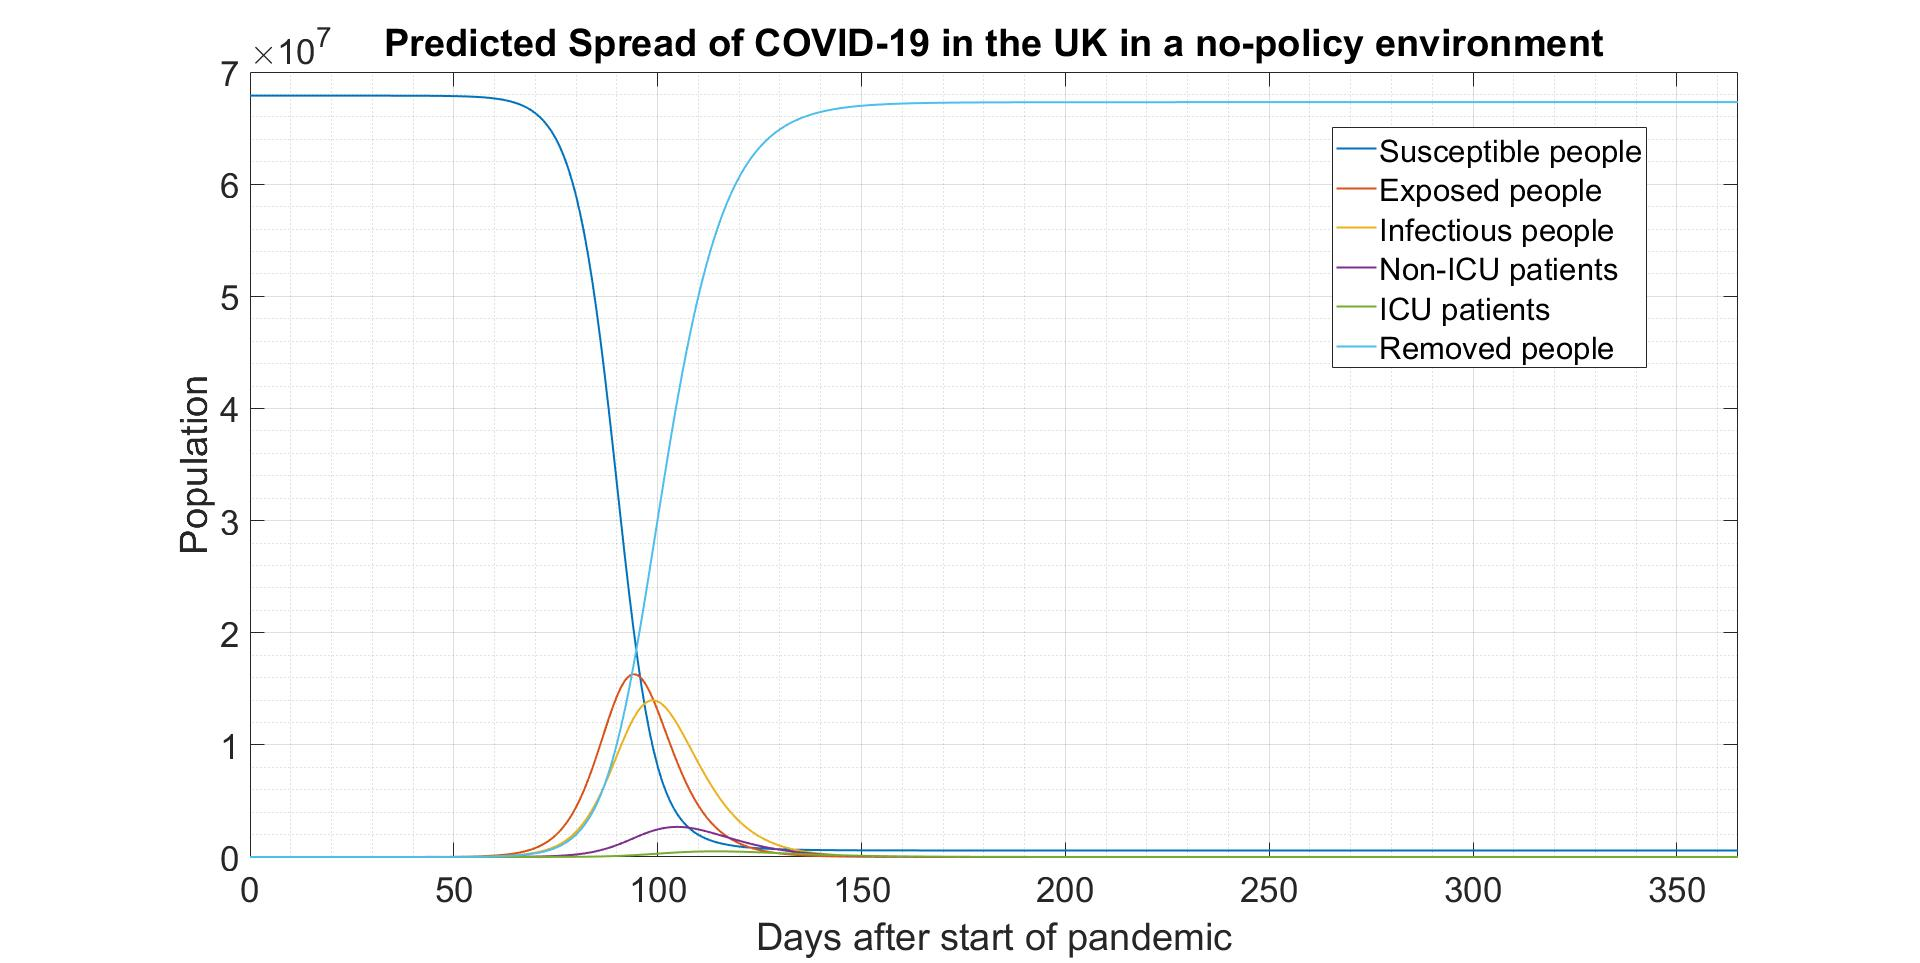
\includegraphics[width=1\textwidth]{No-policySEIHR.jpg} 
\end{center}
\subsection{Hospitialisations in a no-policy environment}
\begin{center}
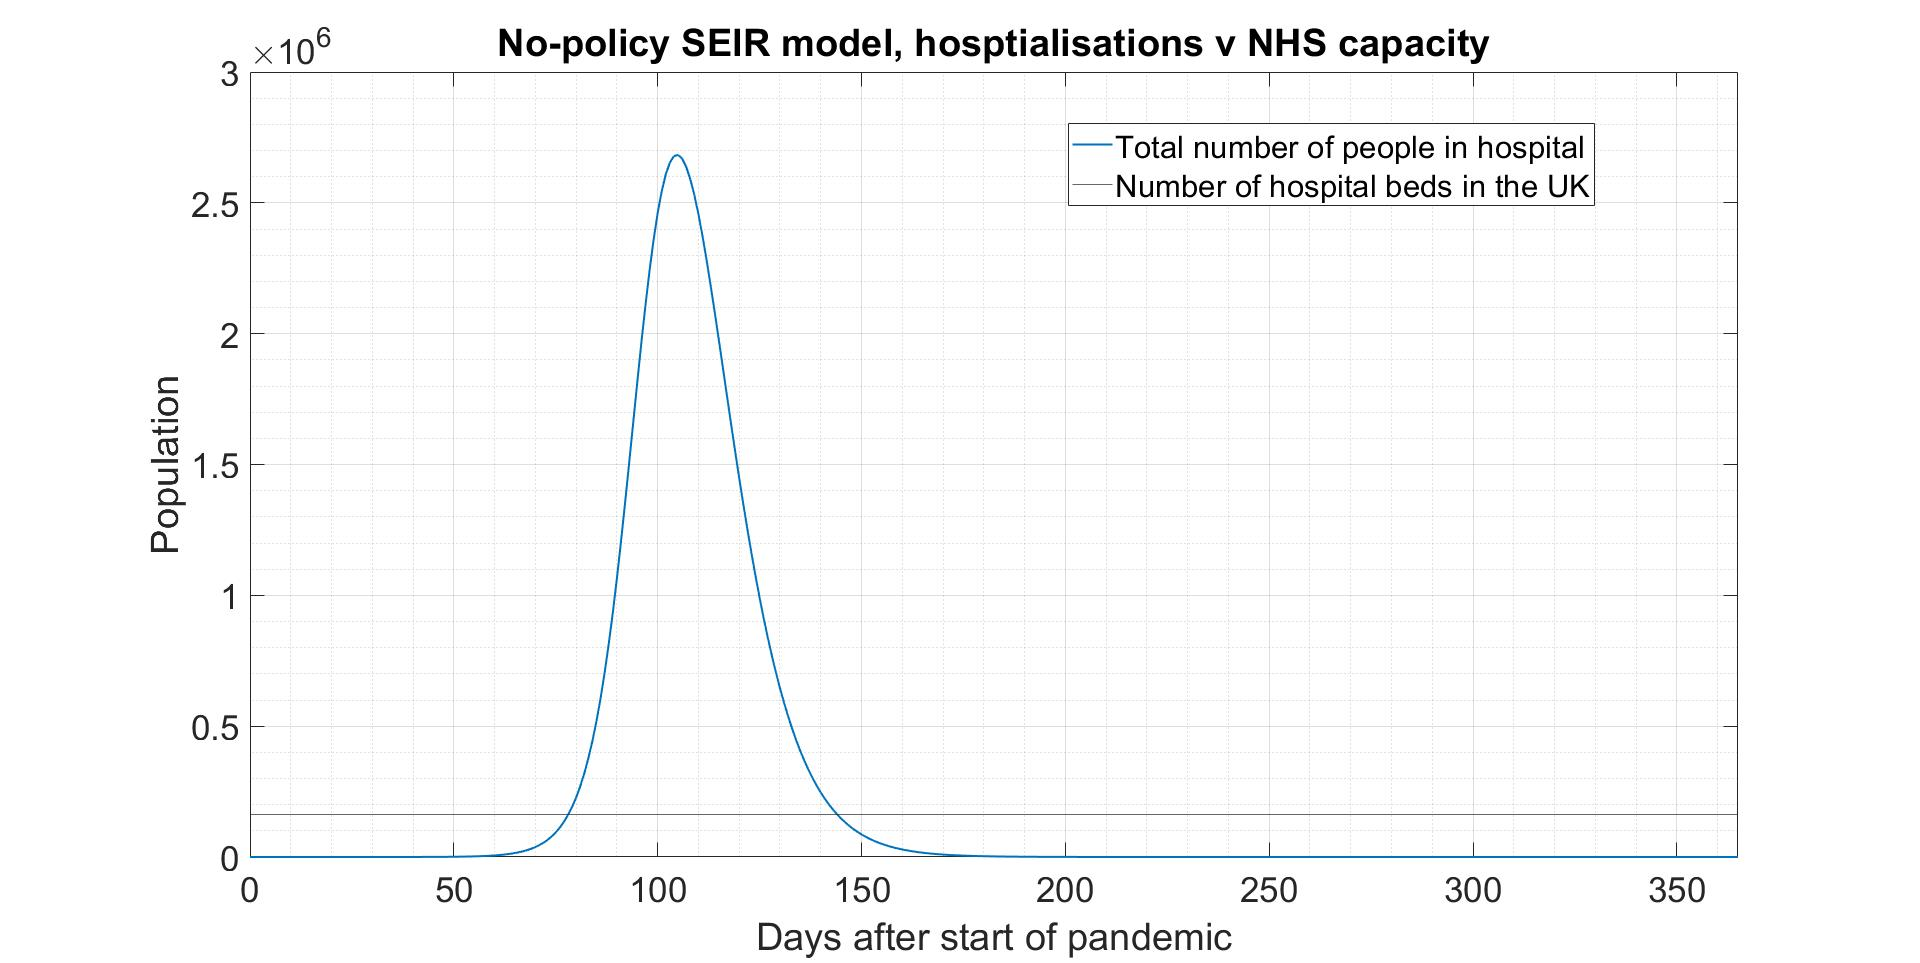
\includegraphics[width=1\textwidth]{No-policyH.jpg} 
\end{center}
\begin{center}
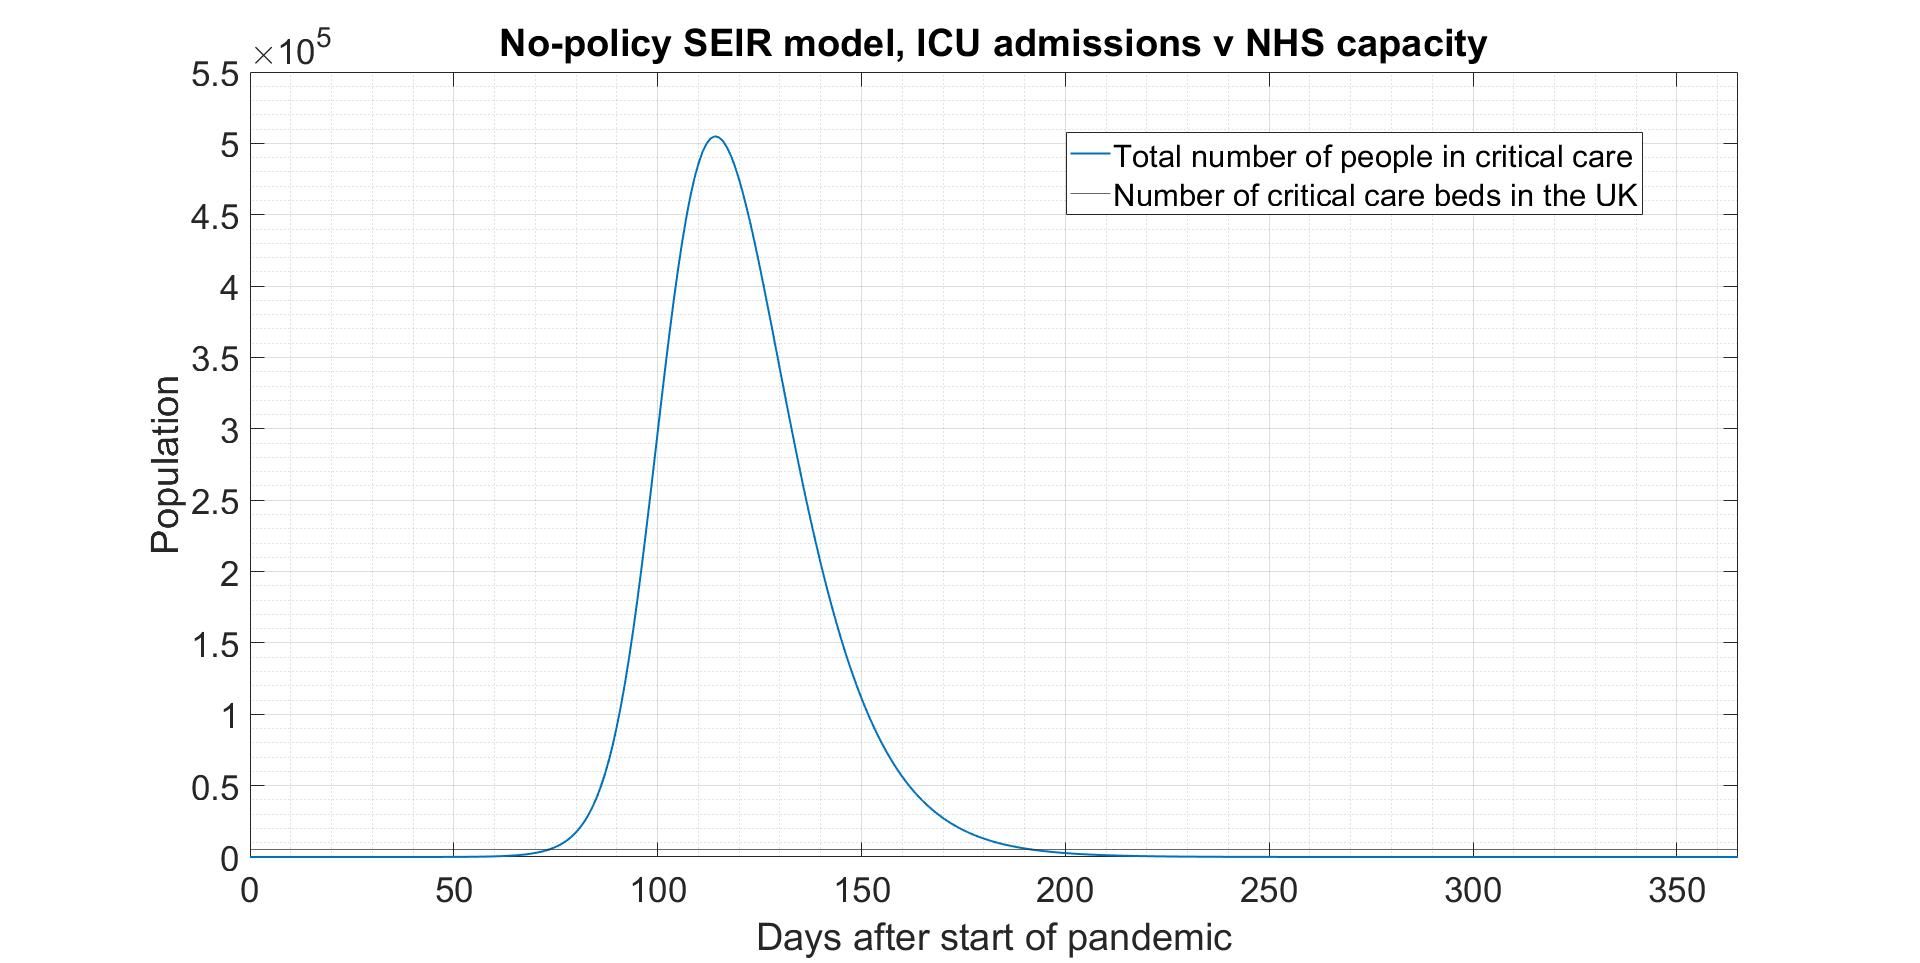
\includegraphics[width=1\textwidth]{No-policyHICU.jpg} 
\end{center}
gknregioehbio
\section{Modelling Strategies}
\subsection{Full Lockdown}
\begin{center}
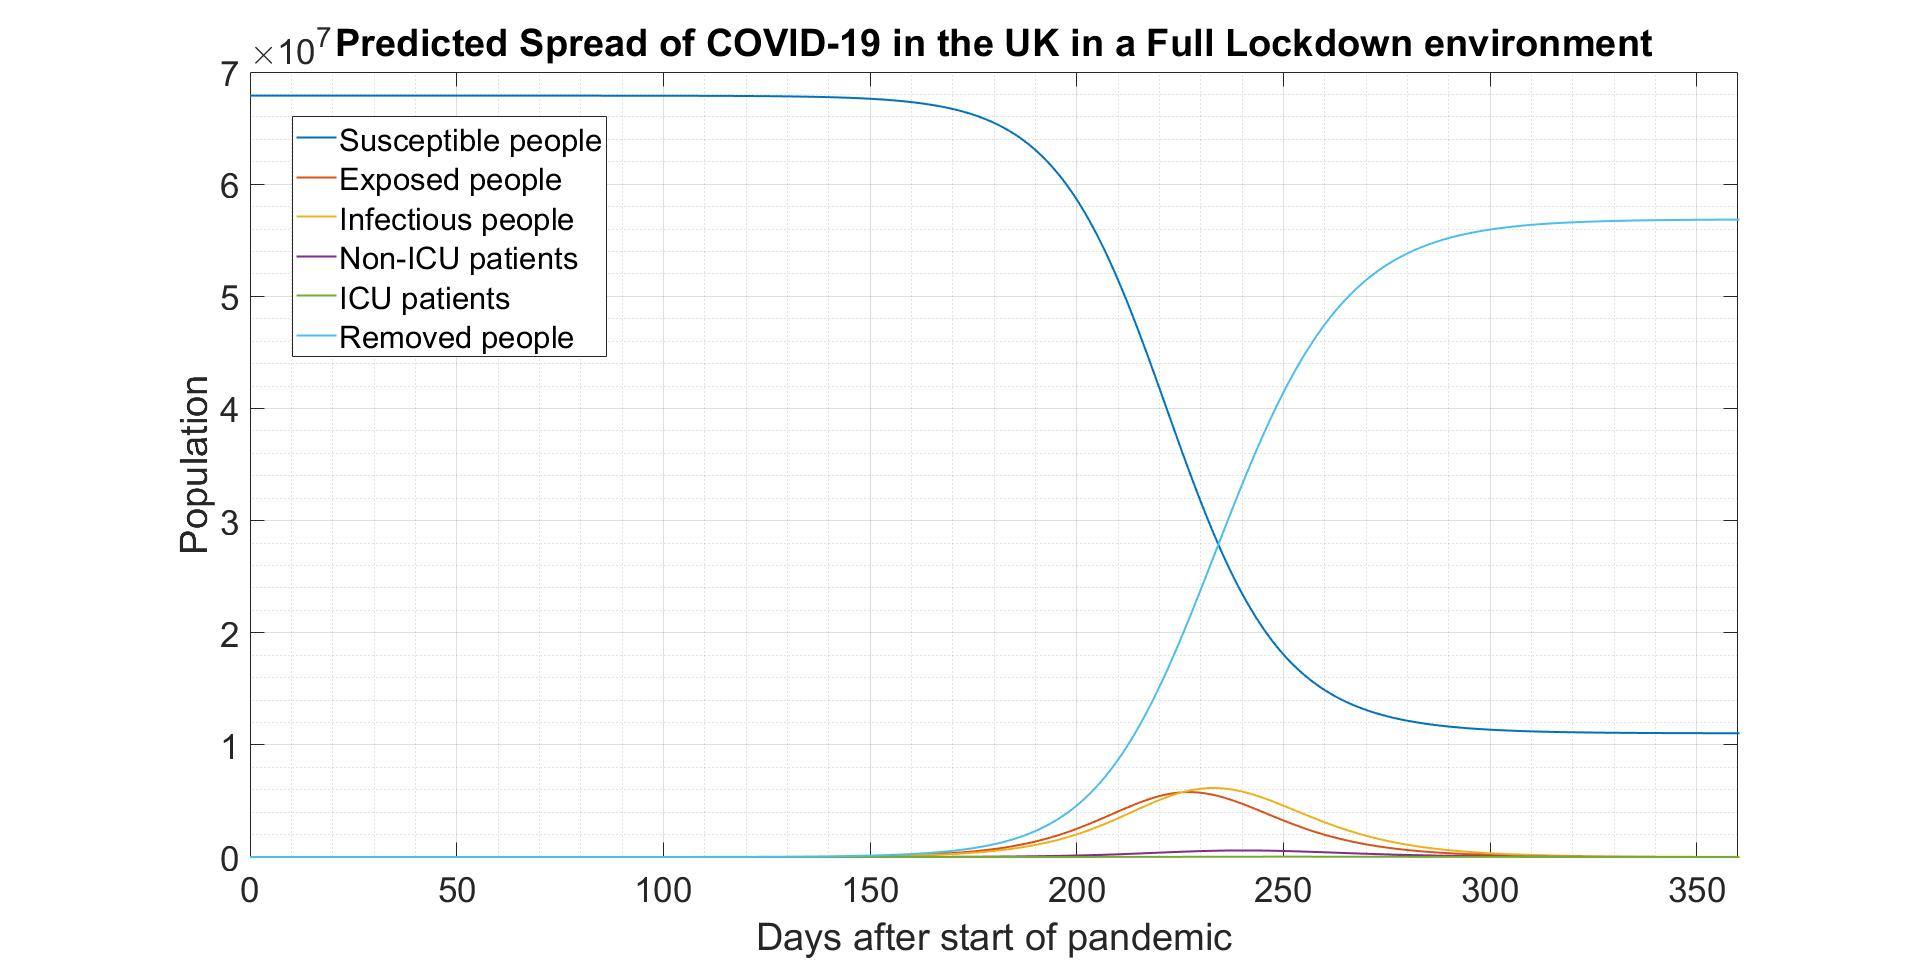
\includegraphics[width=1\textwidth]{FLSEIHR.jpg} 
\end{center}
\begin{center}
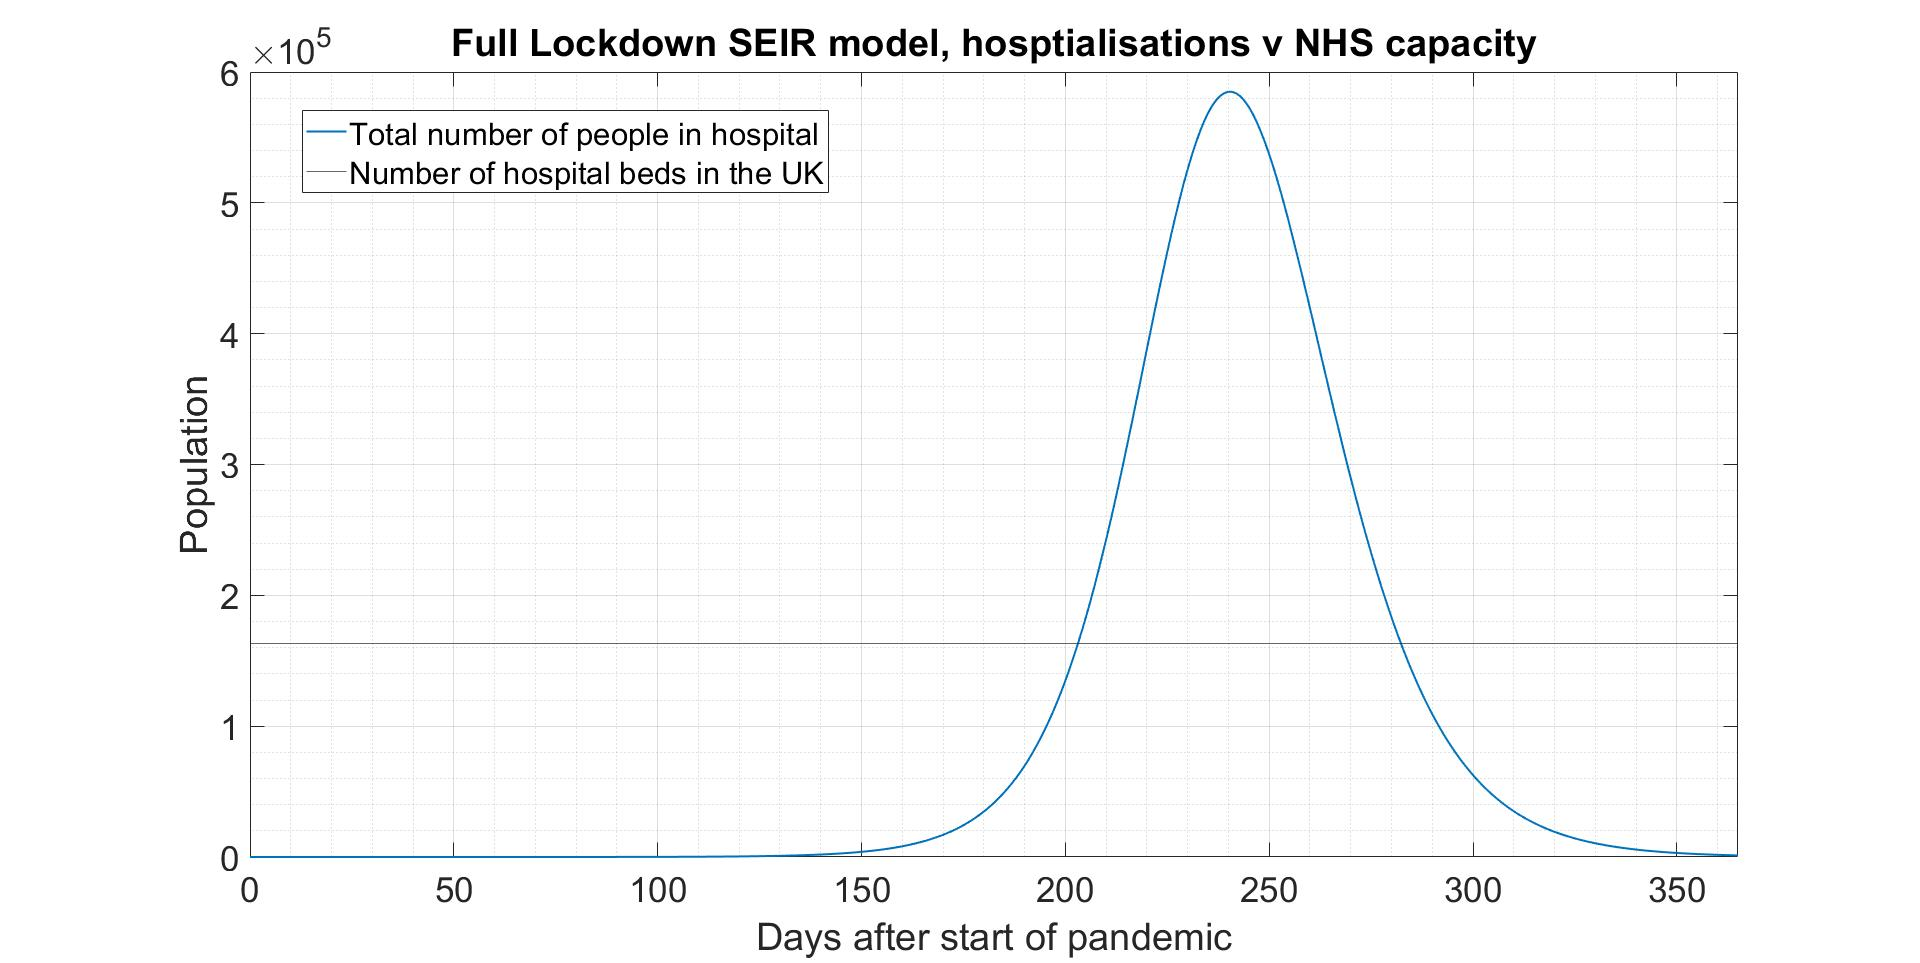
\includegraphics[width=1\textwidth]{FLH.jpg} 
\end{center}
\begin{center}
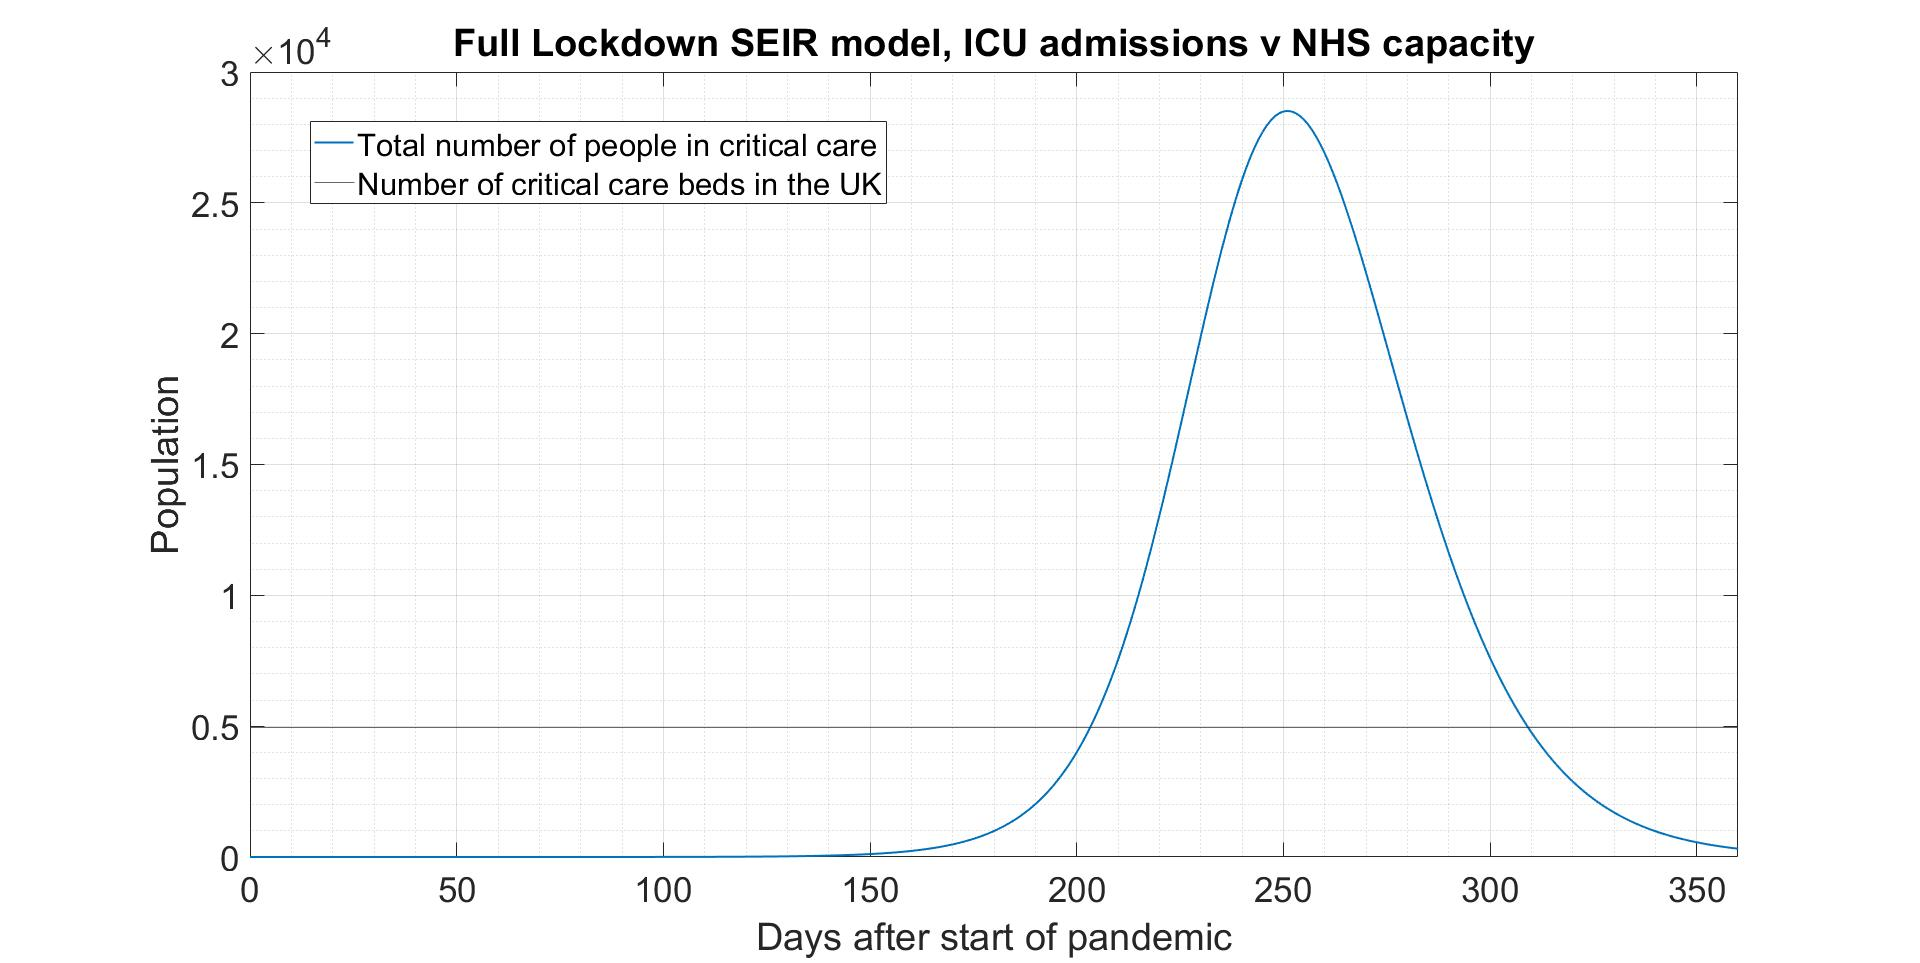
\includegraphics[width=1\textwidth]{FLHICU.jpg} 
\end{center}
\subsection{Rule of Six}
\begin{center}
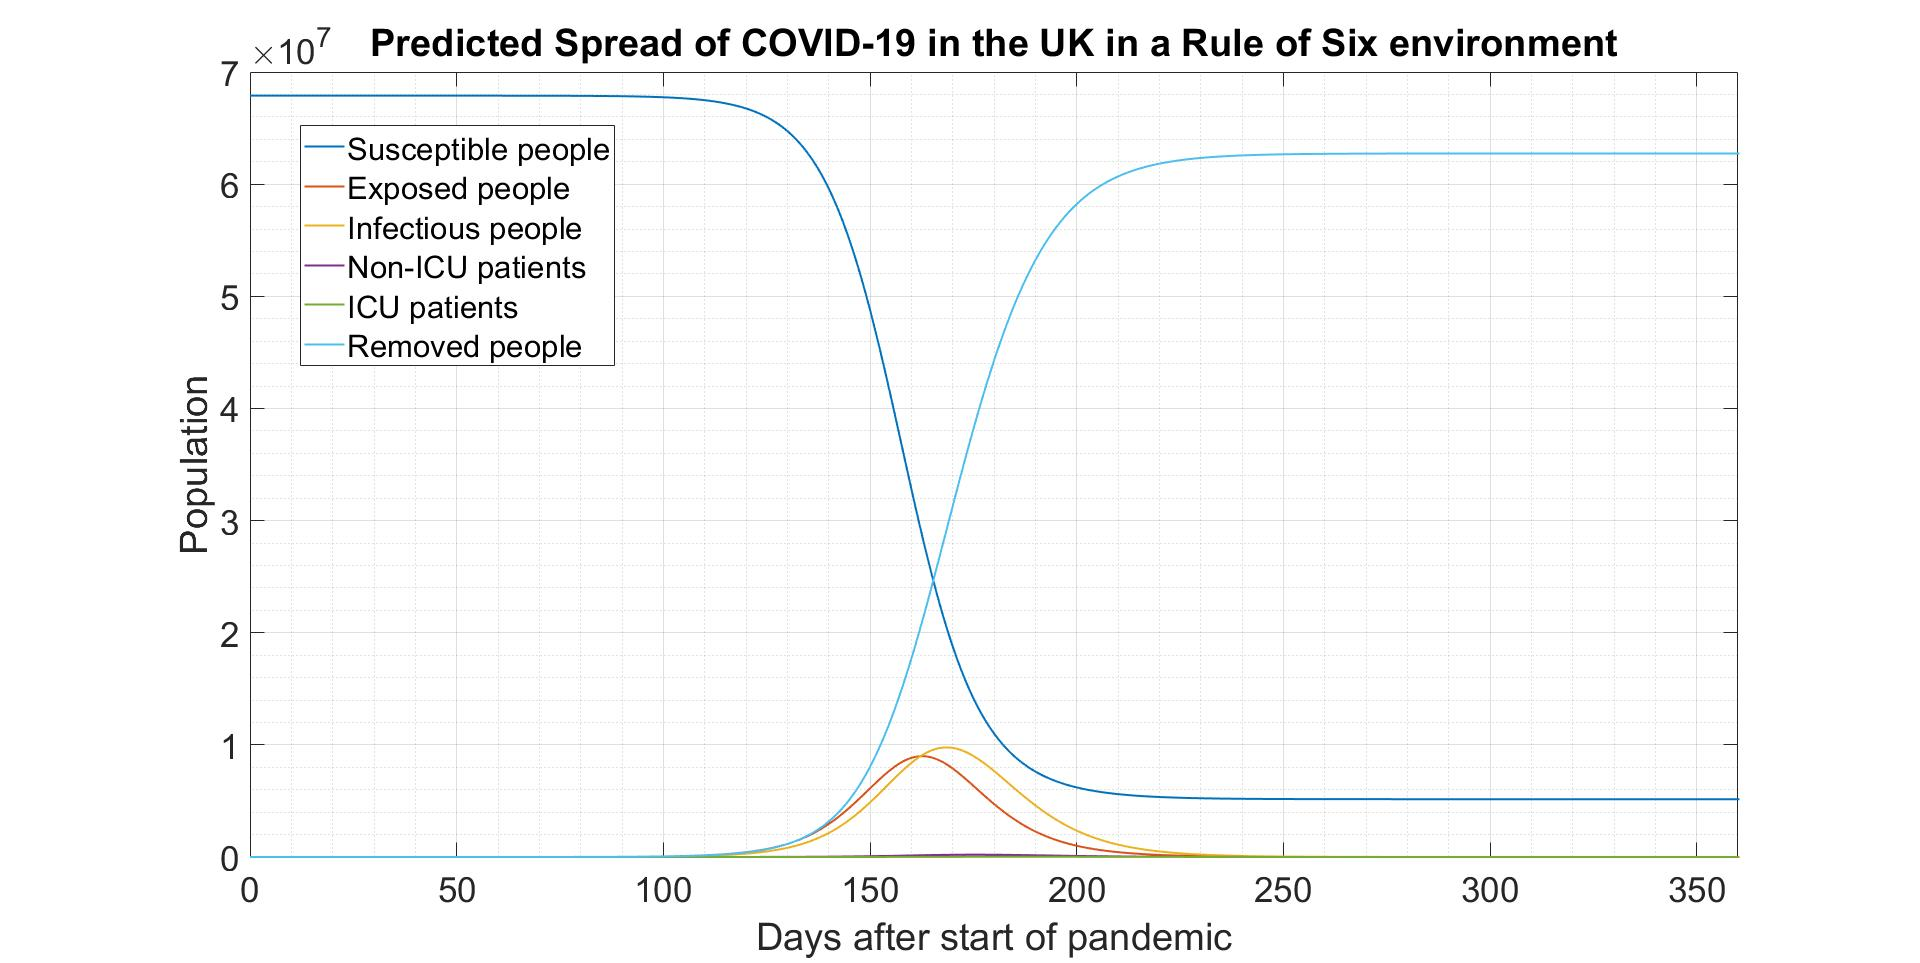
\includegraphics[width=1\textwidth]{ROSSEIHR.jpg} 
\end{center}
\begin{center}
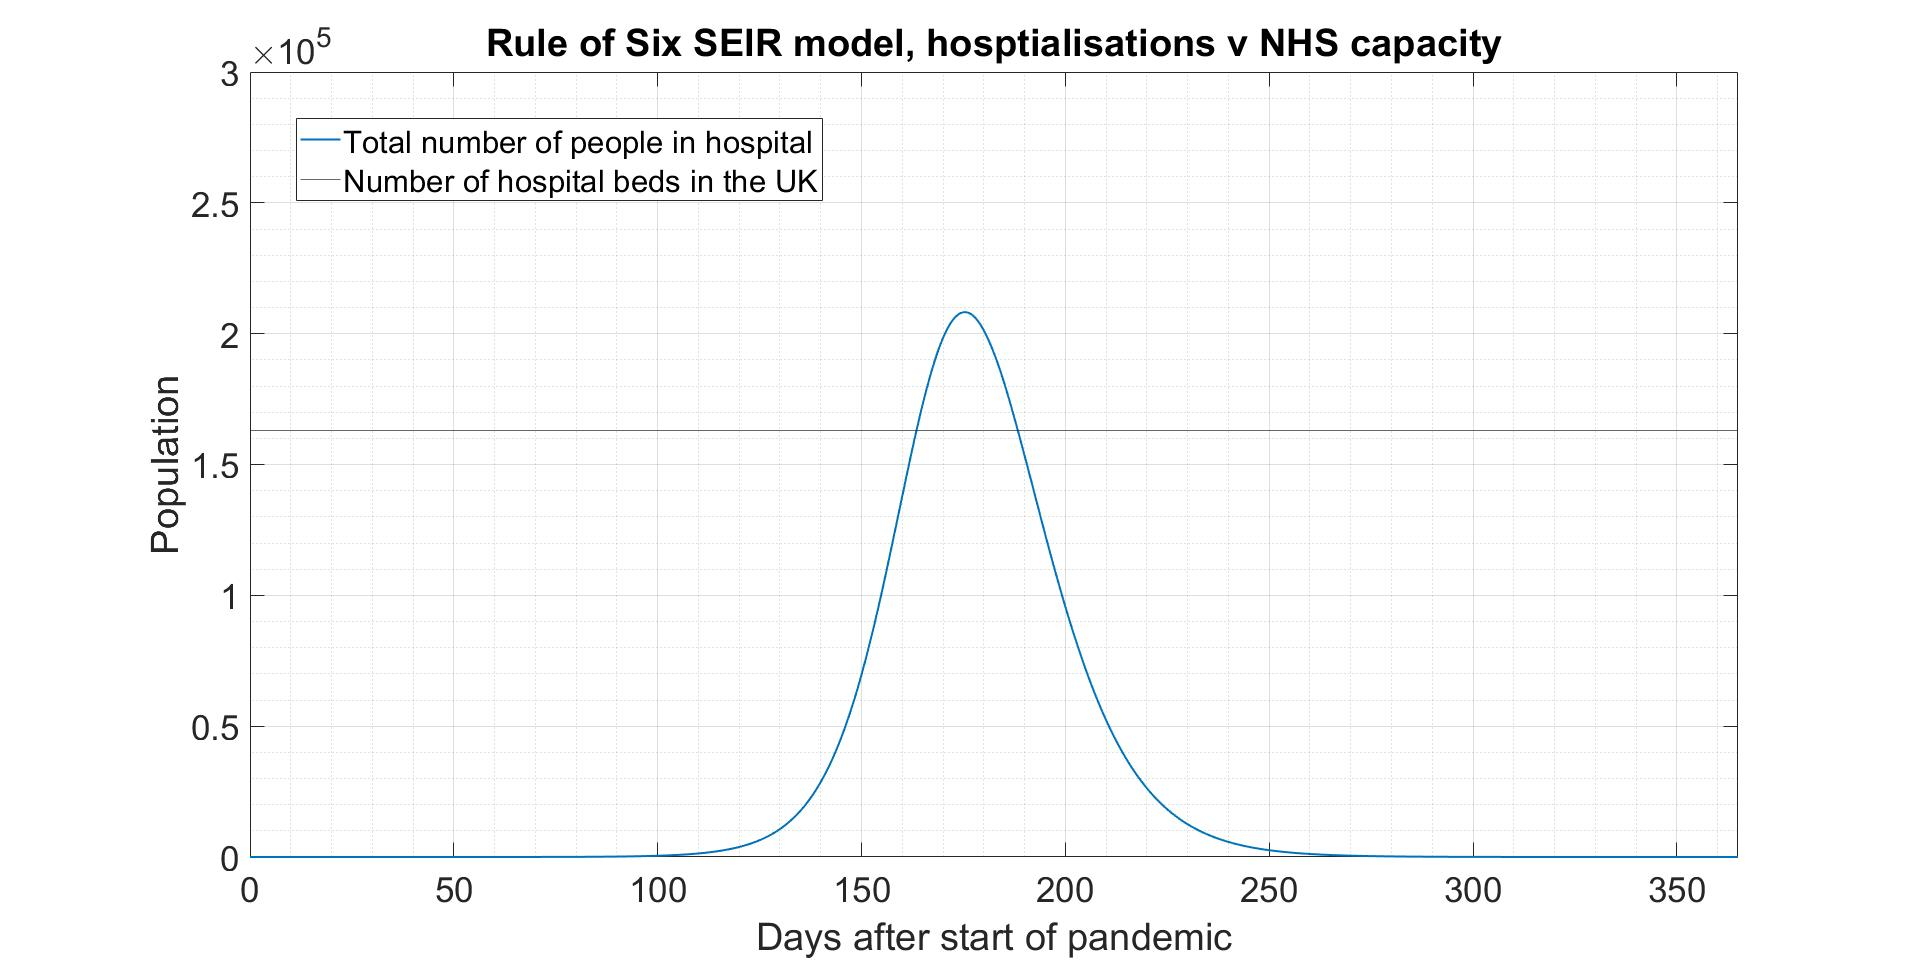
\includegraphics[width=1\textwidth]{ROSH.jpg} 
\end{center}
\begin{center}
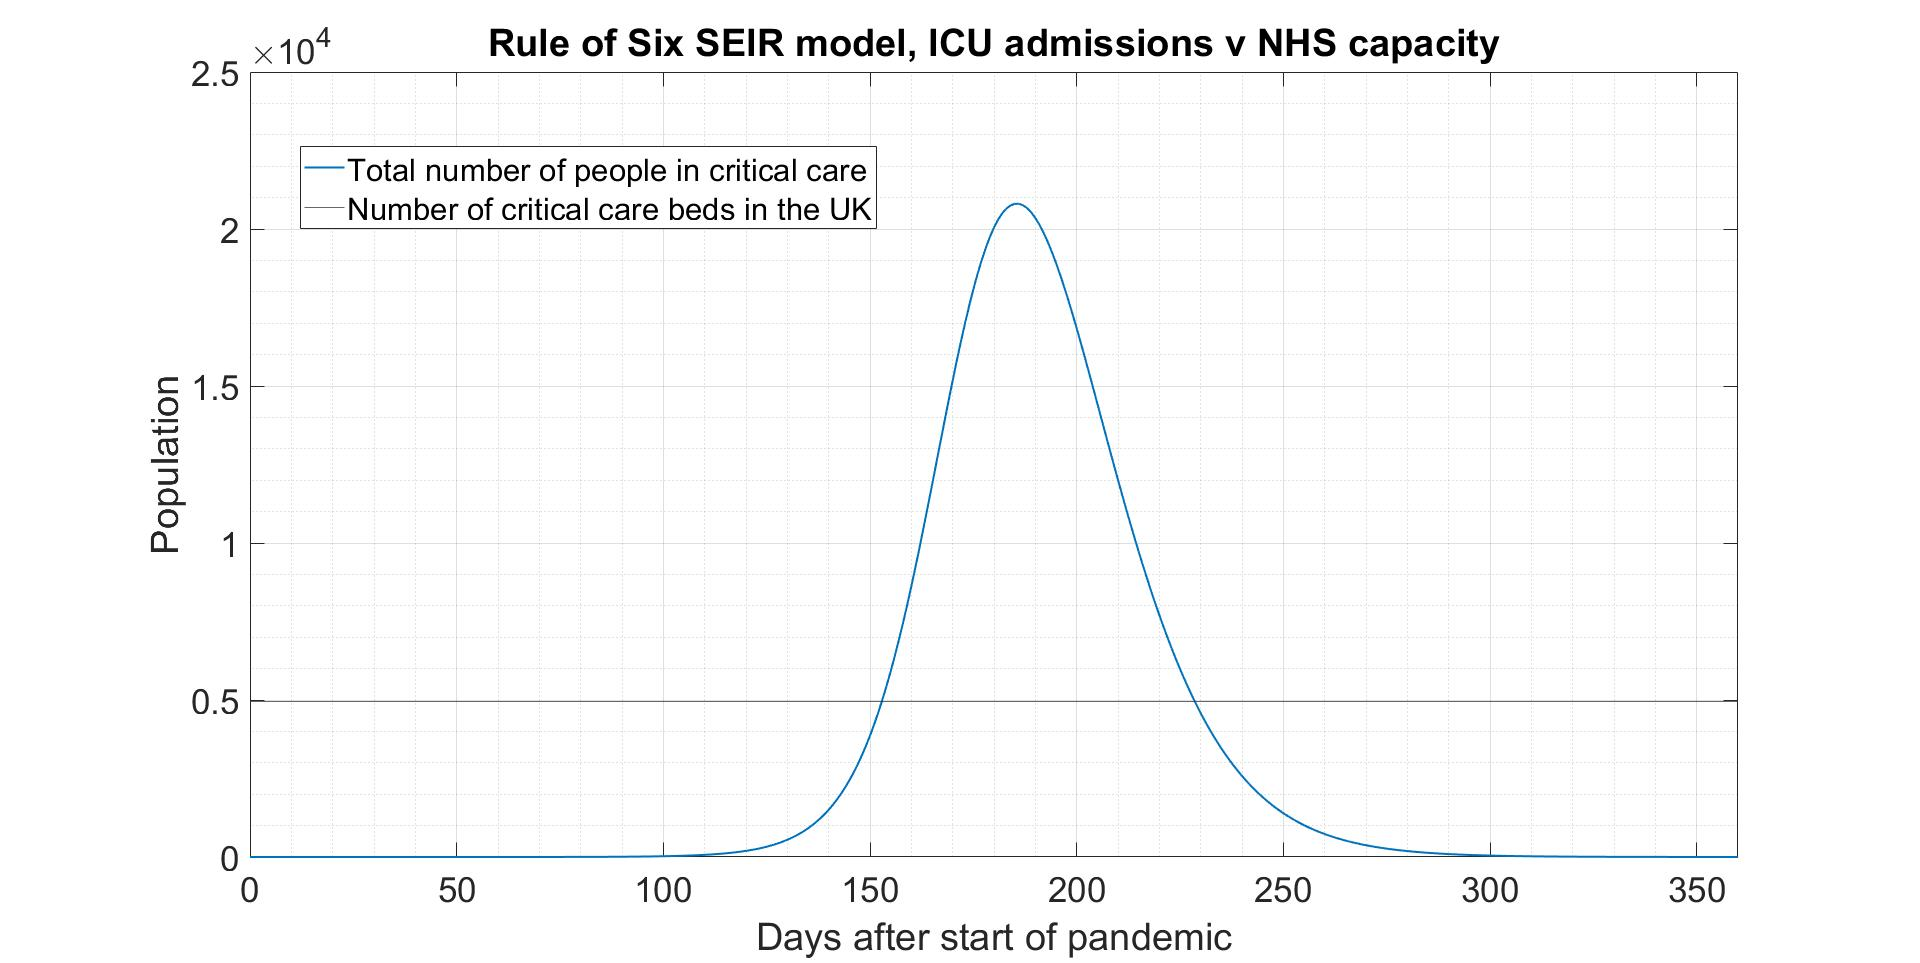
\includegraphics[width=1\textwidth]{ROSHICU.jpg} 
\end{center}
\subsection{Local Lockdowns}
\begin{center}
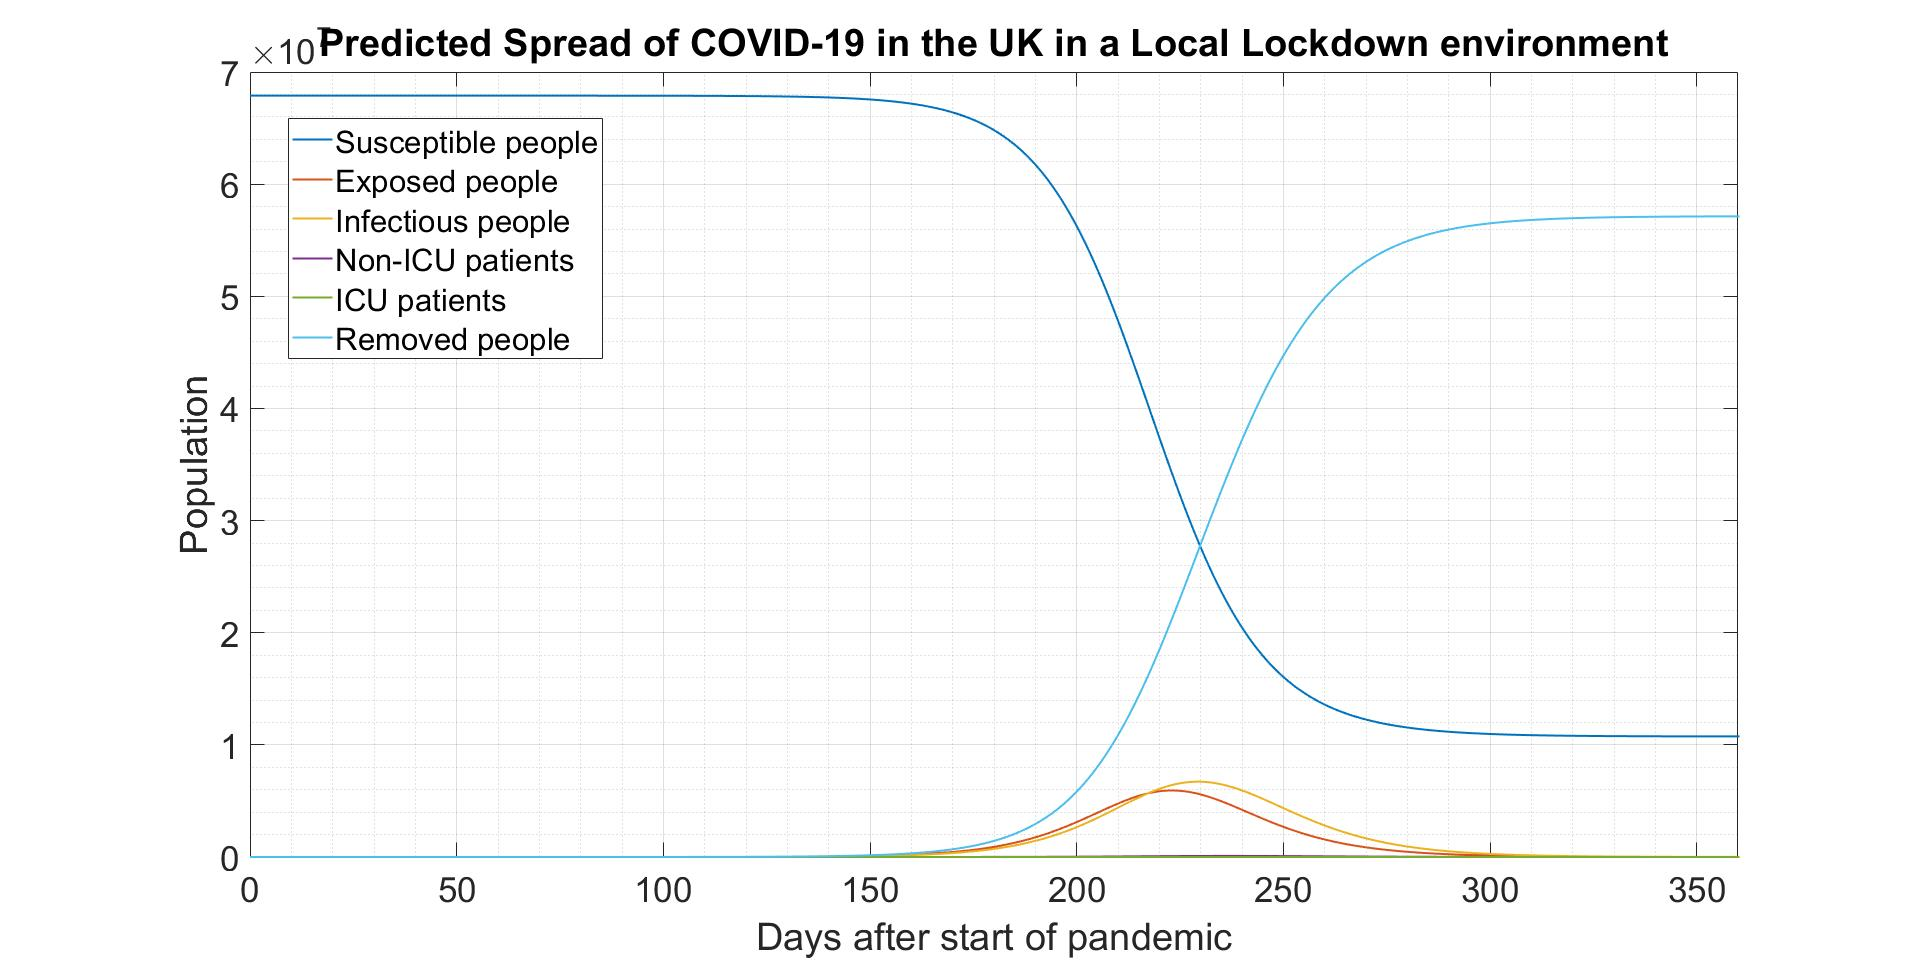
\includegraphics[width=1\textwidth]{LLSEIHR.jpg} 
\end{center}
\begin{center}
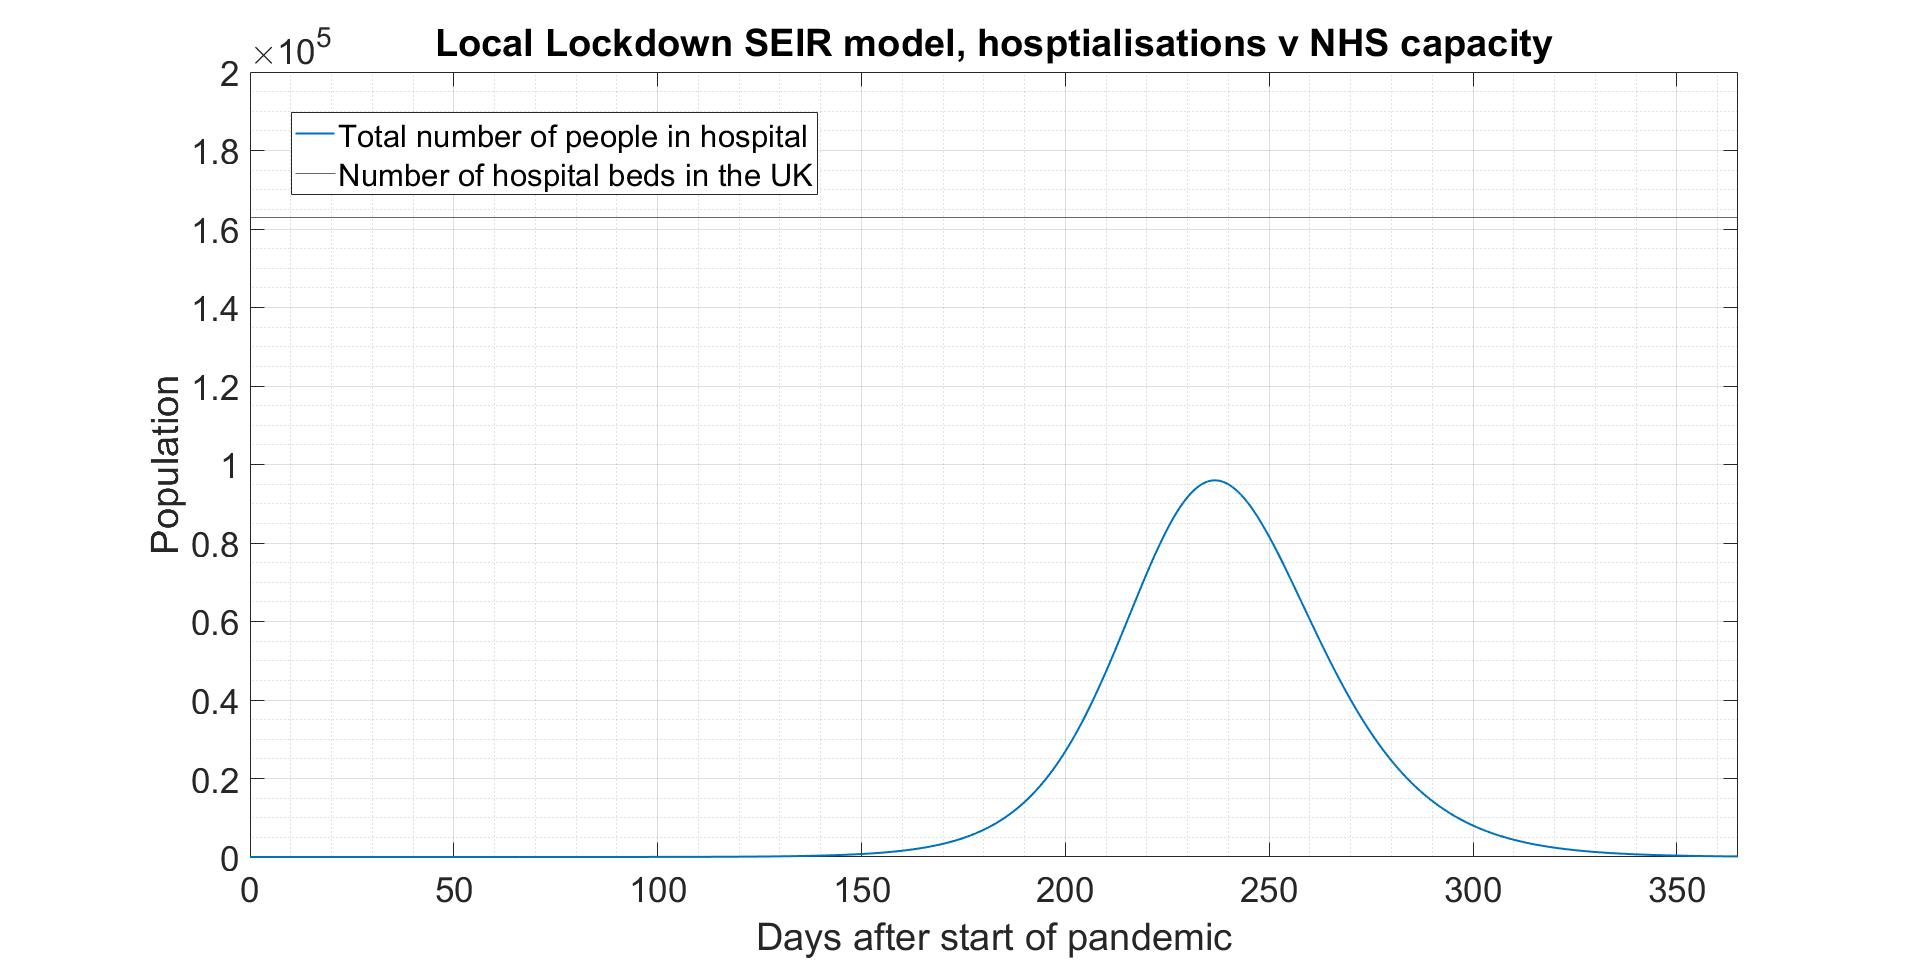
\includegraphics[width=1\textwidth]{LLH.jpg} 
\end{center}
\begin{center}
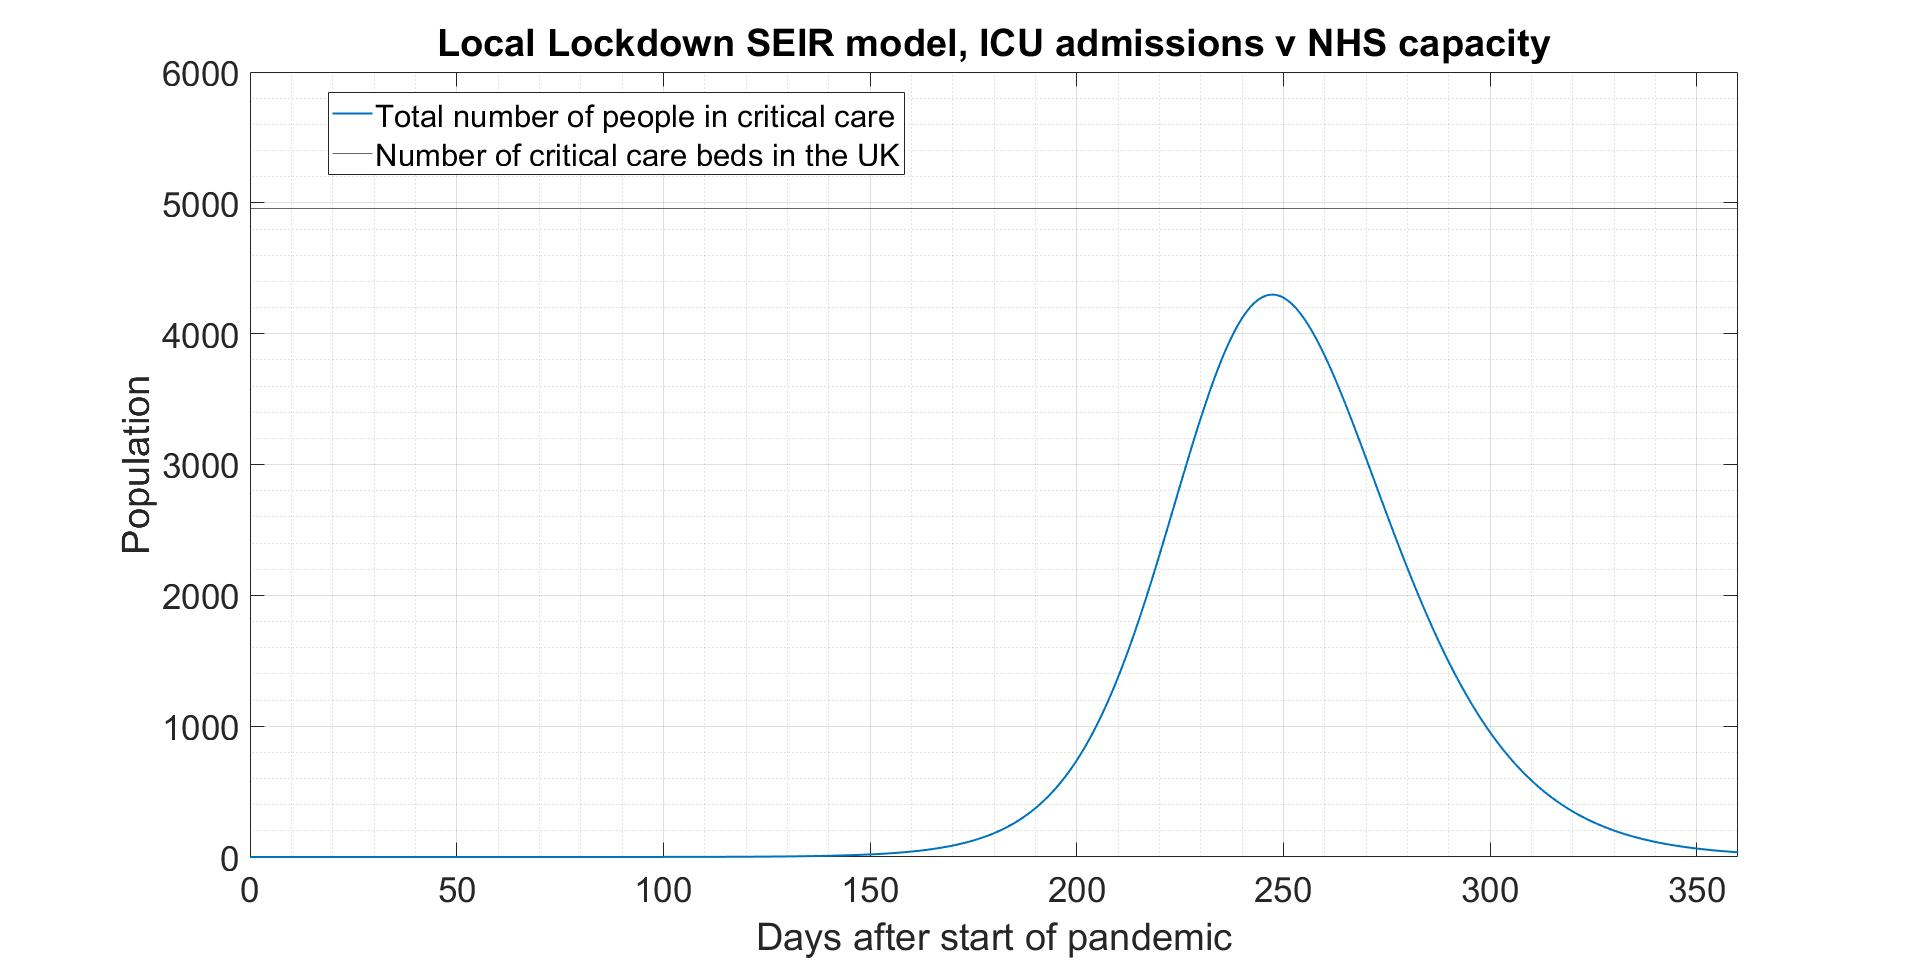
\includegraphics[width=1\textwidth]{LLHICU.jpg} 
\end{center}
\subsection{Vaccinations}
\section{Conclusion}
\subsection{Limitations}
There are many limitations that come with any model, this model is data driven, hence the main limitation is the data. To minimise limitations from the data, I used data from only one source \citep{DataSource} for the sake of consistency between different environments I will be modelling. All parameters are calculated using data, for no-policy and for strategies, using logic would not allow for comparisons. For example, assuming contact reduced by a half in a full lockdown environment and taking half the no-policy parameters for rate of transmissions would guarantee that the lockdown would make a notable change in cases, therefore comparisons will be trivial. \par
Furthermore, using data during the pandemic to model a pandemic from the start will ensure differences in the models that are not due to strategies at the time, however due to which point we are in the pandemic. We know that COVID-19 is more likely to hospitalise elderly citizens in fact, relative to 18-29 year olds, 50-64 year olds are 3 times more likely to be hospitalised by COVID-19, and this risk only increases with 85+ year olds 10 times more likely to be hospitalised by COVID-19\citep{AGE}. Some parts of the UK, which people may call ‘retirement towns’ have a greater elderly population, and if COVID-19 is currently peaking in said area, then there will be more hospitalisations overall. This is just one case of why data may not accurately represent strategy effectiveness. Moreover, in these models I have not considered the existence of variants, which have formed throughout the pandemic, data from later may be affected by this given some variants have a greater rate of transmission compared to other variants, which again is unrelated to the strategy \par
Other reasons include: lack of people living in accordance to government guidelines, I have assumed that majority of people do comply with assumption $6$ in order to allow for comparisons, time of the year: Christmas holidays would encourage more people to see families, etc.  Again, we must consider limitations due to age, the UK is known for having an elderly population, as mentioned this naturally increases the hospitalisations regardless of effectiveness of strategy. \par
In addition, these models only show one peak, this is due to assumption $7$, For the sake of a simplified model this assumption was necessary, but as we have observed from data this is not the case shown by multiple peaks due to population structure and reinfection. Due to lack of data on the rate of reinfection, I have not included this in my model by assumption $4$. But this does not limit the ability to make comparisons, once we consider these models to display worst case of spread, we can discard the effect on conclusion. \par
\subsection{When are we expected to reach herd immunity?}Herd immunity in line with the given models is reached when all the susceptible population is removed, by assumption $3$ ‘All individuals are equally susceptible to COVID-19, and the whole population is considered susceptible at the start of the pandemic’ and assumption $4$ ‘Individuals that are recovered cannot be reinfected i.e., immunity is assumed’ combined implies that once all susceptible people are removed, the whole population is removed and therefore immune. However, we know that this is not the case, since in reality, reinfection is possible, immunity seems to be temporary, and new variants of COVID-19 are continuously being formed due to the global spread. These new variants may be more resistant to immunity hence may be able to infect those who were even more recently infected. For now, vaccines have shown to be effective against all variants so far, hence the spread of vaccines may be the key to herd immunity. \par
In relation to these models herd immunity is given by the steady state of the system $(1)$:
\begin{equation}
\begin{aligned}
\frac{dS}{dt}&=0\\
\frac{dE}{dt}&= 0 \\
\frac{dI}{dt}&= 0 \\
\frac{dH}{dt}&= 0\\
\frac{dH_{ICU}}{dt}&= 0 \\
\frac{dR}{dt}&=0 \\
\end{aligned}
\end{equation}
The steady state $(2)$ gives an endemic state, there is no change in any variables, the pandemic is over. For each model the endemic state will be different as there will be different parameters at play. This is key to comparing strategies as the sooner herd immunity occurs, the sooner the population will return to normality.
\subsection{Comparisons}
\subsection{Conclusions}
\newpage
\bibliography{mybib}
\bibliographystyle{unsrt}
\section{Appendices}
\lstinputlisting[style=Matlab-editor,caption={No-policy environment function with matrix of ODEs} ]{ode_fun_UKcovid.m}
\lstinputlisting[style=Matlab-editor,caption={No-policy environment end of COVID-19 function} ]{findEnd.m}
\lstinputlisting[style=Matlab-editor,caption={No-policy environment using initial data on COVID-19} ]{SEIRMODEL.m}
\begin{verbatim}
COVID-19 is eradicated when, t=270, S=5.816017e+05, R=6.730838e+07
\end{verbatim}
\end{document}